


\subsubsection{Exotic  decays of the Higgs to $2b2\mu$}
\begin{center}
 {David Curtin$^{1}$, Rouven Essig$^{2}$, and Yi-Ming Zhong$^{3}$\\
}
\centerline{{\it $^{1}$Department of Physics, University of Toronto, Toronto, ON M5S 1A7, Canada}}
\centerline{{\it  $^{2}$C.N. Yang Institute for Theoretical Physics, Stony Brook University, Stony Brook, NY 11794, USA}}
\centerline{{\it  $^{3}$Physics Department, Boston University, Boston, MA 02215, USA}}
\end{center}
Here we assess the potential of an exotic Higgs decay search for $h \to 2X \to b\bar{b}\mu^+ \mu^-$ to constrain theories with light CP-even ($X = s$) and CP-odd ($X = a$) singlet scalars.  This decay channel may represent the best discovery avenue for many models, such as the 2HDM model with an additional complex scalar singlet (2HDM+S). It has competitive reach, and is less reliant on low-$p_{\rm T}$ $b-$ and $\tau-$reconstruction compared to other channels like $4b$, $4\tau$, and $2\tau2\mu$. 


To estimate the reach of $h \to 2X \to b\bar{b}\mu^+ \mu^-$ search at the 14 TeV LHC, we take $X =a$ for simplicity. (Results for $X=s$ should be similar.) The dominant backgrounds are Drell-Yan (DY) production with associated jets, \ie $Z/\gamma^*+2b/2c/2j$, where $Z/\gamma^*$ produces a muon pair. A secondary background arises from $t\bar t$ production. Backgrounds from diboson production ($ZZ, WW, WZ$) have small enough cross sections so that we can neglect them. It is also possible for QCD multi-jet events, with two jets being mis-identified as muons, to contribute to the background. We find this can be neglect for analysis with $b$-tags. Signal, as well as DY and $t\bar t$ backgrounds, are simulated at LO by \texttt{Sherpa 2.1.1}~\cite{Gleisberg:2008ta} for $\sqrt{s}=14$ TeV with the CT10 PDF, and matched up to three jets. The Higgs production cross section for the signal is normalized to the NLO gluon-fusion cross section $\sigma_{ggF} \simeq 49.47 \pb$~\cite{Dittmaier:2011ti}.  



Two types of analyses have been included. A conventional analysis use standard anti-$k_t$ jets with a jet radius of $R\sim 0.4$. Two $b$-tags at 70\% $b$-tagging efficiency working point~\cite{ATLAS:2014cal}  are imposed to the final states. A missing transverse energy cut of $\slashed{E}_T < 30 \UGeV$ suppresses $t \bar t$ background. In addition we make use of the double-resonance structure of the signal by imposing invariant mass cuts 
\begin{align}
|m_{b_1 b_2 \mu_1 \mu_2}-m_h|< 15\UGeV,\quad |m_{b_1 b_2}-m_a|< 15\UGeV,\quad|m_{\mu_1\mu_2}-m_a| < 1\UGeV,
\end{align}
separately for each $m_a$. After passing above cuts, we then perform a simple counting experiments to estimate the reach. The expected bounds are approximately independent of scalar mass for $m_a \geq 30 \UGeV$. For $m_a < 20 \UGeV$, the signal efficiency drops dramatically because the two $b$'s from the $a$-decay become collimated. Instead we adopt the mass drop tagger (MDT)~\cite{Butterworth:2008sd}, a jet substructure technique, to improve the search sensitivity for the low -$m_a$ region. After clustering a $b$-tagged C/A  jet with a jet radius of $R=0.8$, we resolve its hardest subjets that satisfy the MDT criteria ($\mu < 0.67$, $y>0.09$) by undoing the last step of the C/A clustering. We then apply the same missing energy and invariant mass cuts to the subjets as the conventional analysis.

The results of the combined substructure and conventional analysis are shown in Fig.~\ref{bbmumu}. It shows a fairly flat sensitivity of  $\mathrm{Br}(h \to 2a \to 2b2\mu) \lesssim \text{few}\times10^{-4}$ for 14 TeV LHC with 30 ${\rm fb}^{-1}$ data in the range $15\UGeV \leq m_a \leq 60 \UGeV$. With either 300 or 3000 ${\rm fb}^{-1}$ of data, the projected sensitivity increases to  $10^{-4}$, and $\text{few}\times 10^{-5}$, respectively. For HE-LHC (27 TeV with $15\ab$), we expected the number of signal and DY background events to be respectively increased by a factor of $\sim15$ and $\sim12$ in comparison with those of the HL-LHC (14 TeV with $3\ab$). This yield reach estimates for HE-LHC to be 
$\lesssim 10^{-5}$, i.e., a factor of $15/\sqrt{12}\approx 4$ better than those of the HL-LHC. In the same plot, we also show the 95\% CL bounds from 13 TeV ATLAS analysis with 36.1 ${\rm fb}^{-1}$ data~\cite{Aaboud:2018esj} as the black shaded region (assuming the Higgs production cross section to be the same as the SM prediction). For a range of $m_a$ values, the ATLAS bounds are better than our projections  by a factor of a few. This may due to more dedicated analysis techniques such as kinematic-likelihood fit~\cite{Aaboud:2018esj}, which improves the invariant mass resolutions. Based on above comparison, we expect the real HL-LHC and HE-LHC reach should be better than our conservative projections. 



\begin{figure}[h]
\begin{center}
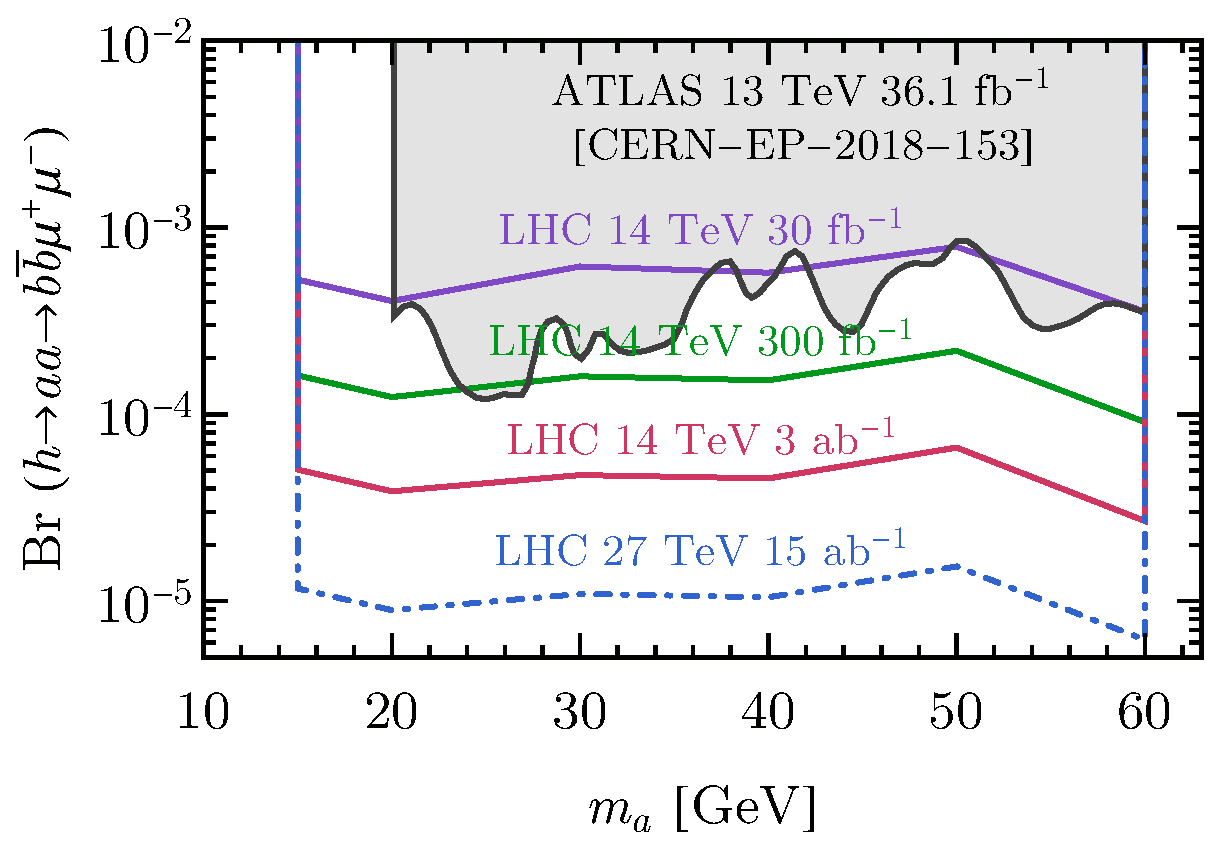
\includegraphics[width=0.65\textwidth]{\main/section9/sensitivity-2.pdf}
\caption{\small Combined $95\%$ CL projected reaches on $\Br(h\to aa \to b\bar{b}\mu^+ \mu^-)$ for 30 (purple), 300 (green), and 3000 (red) ${\rm fb}^{-1}$ at 14 TeV~\cite{Curtin:2014pda} and 15 $\ab$ at 27 TeV (dash-dotted blue). The 95\% CL upper limits from  13 TeV ATLAS with 36.1 ${\rm fb}^{-1}$ data~\cite{Aaboud:2018esj} is shown as the black shaded region.}
\label{bbmumu}
\end{center}
\end{figure}
